\chapter{Teorema CA}

\newpage
\section{Relaciones no aplicación}
Uno de las herramientas de este trabajo van a ser relaciones que no son aplicación: simples correspondencias. Y no serán 'función', porque por cada elemento del conjunto Dominio, a veces, tendremos relacionados más de un elemento del conjunto Imagen. Y no serán varios elementos dentro de un conjunto, sino que serán varios pares de la relación, cuyo elemento del Dominio es el mismo, pero cambian los elementos del conjunto Imagen, en cada par.

Por ejemplo:

\noindent Siendo el conjunto $X=\{a,b,c\}$ y el conjunto $Y=\{1,2,3,4,5,6,7,8,9\}$, y una relación $r:X \rightarrow Y$, los pares no serán del estilo:\\
$a \rightarrow \{1,2\}$, pues esto no sería una relación entre X e Y, sino entre X y un subconjunto de P(Y).\\\\
\noindent Sino que serán del estilo:\\
$a \rightarrow 1$\\
$a \rightarrow 2$\\\\
\noindent Formándose los pares (a,1) y (a,2)

No serán herramientas exclusivas, pues según el caso, usaremos inyecciones, biyecciones, o cualquier otra herramienta que nos permita obtener deducciones sobre los cardinales de los conjuntos envueltos. Siempre explicando el motivo por el cual nos permitimos la licencia de usar esa herramienta y no las conocidas. 

NO IMPORTA que las herramientas que usemos sean enrevesadas o poco elegantes, ni incluso que existan alternativas más sencillas... simplemente deben ser correctas y estar lo mejor definidas posible.

\newpage
\section{Concepto de Pack}
\noindent
Sea $f:X \rightarrow Y$\\ 
correspondencia entre conjuntos cualesquiera.\\

\noindent 
Sea $a \in X$ definimos:\\
$f(a) = \{ b \in Y / f(a) = b \}$\\ 
el conjunto imagen mediante la correspondencia $f$ del elemento $a$ de $X$.\\

\noindent 
Llamamos 'Pack' de $a$ a todo subconjunto NO VACÍO de $f(a)$.

\newpage
\section{Teorema CA}
 
Sean los conjuntos con cardinal transfinito cualesquiera:\\\\
$A = \{ a_{1}, a_{2}, ... , a_{n}, ... \}$\\
$B = \{ b_{1}, b_{2}, ... , b_{n}, ... \}$\\\\
Con $b_{i} = \{ c_{i1}, c_{i2}, ..., c_{ir}, ... \}$ \\\\
Siendo \textbf{todos} los $b_{i}$ disjuntos entre sí.\\

Hacemos la biyección de A en B tal que:\\\\
$f: A \rightarrow B$\\
$\:\:a_{i} \rightarrow f(a_{i})=b_{i}$\\

Es evidente que es una biyección.\\

Está \textbf{bien definida}:\\
$\forall a_{i} \in A$,  $\exists f(a_{i}) = b_{i} \in B$

Es \textbf{aplicación}:\\
Si $a_{i}=a_{j} \:\:\:\Rightarrow\:\:\: i=j$\\
Y esto implicaría\\
$f(a_{i}) = b_{i} = b_{j} = f(a_{j})$\\
Por lo tanto es aplicación.

Es \textbf{inyectiva}:\\
Si $f(a_{i}) = f(a_{j}) \:\:\:\Rightarrow\:\:\: b_{i}=b_{j}$\\
Como los Packs son disjuntos $\Rightarrow i=j \:\:\:\Rightarrow\:\:\:a_{i}=a_{j}$

Es \textbf{sobreyectiva}:\\
$\forall b_{i} \in B: \: b_{i} = \{c_{i1}, c_{i2}, ... , c_{ir}, ... \}$\\
$\exists a_{i}: \: f(a_{i}) = b_{i}$\\
Por lo tanto es biyectiva.

Como $f(a_{i}) = b_{i} = \{c_{i1}, c_{i2}, ... , c_{ir}, ... \}$. Entonces el $|A| \ngtr |B|$, aunque no sea biyección.
\newpage
Por ejemplo, si con la misma relación:
\begin{figure}[h!]
	%width=\textwidth
	%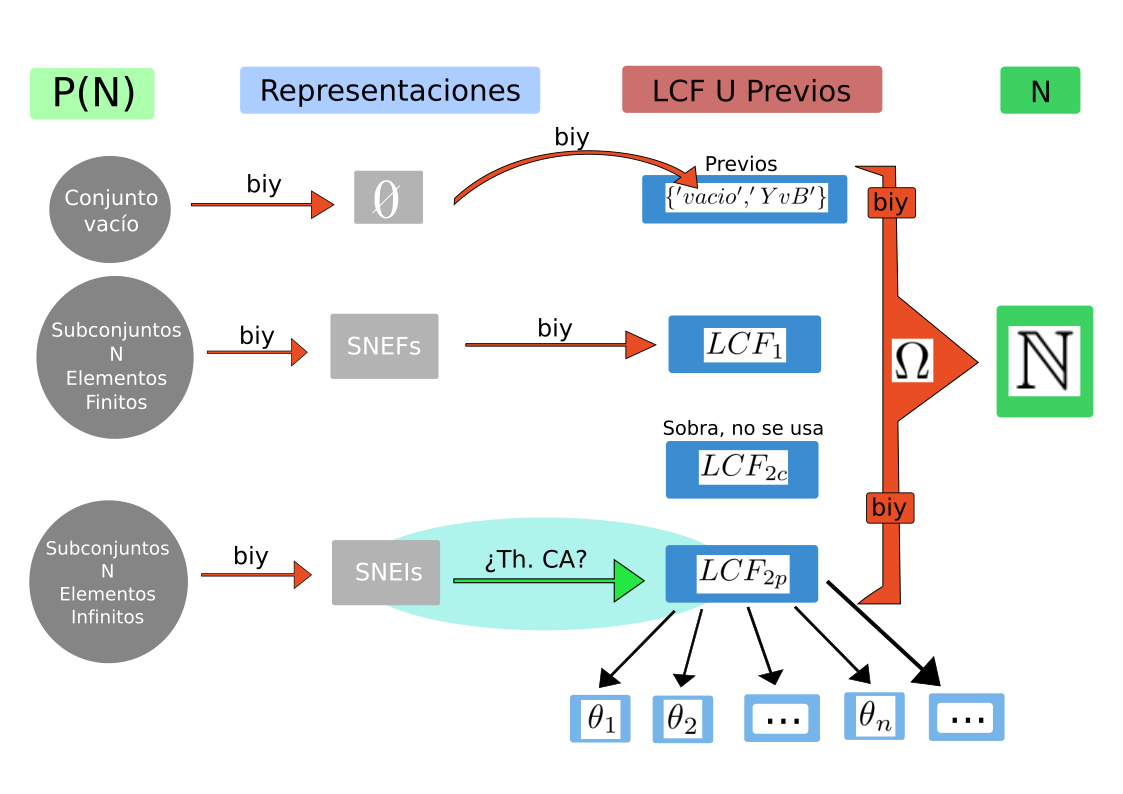
\includegraphics[ scale=0.7, angle=90]{EsquemaRelaciones}%
	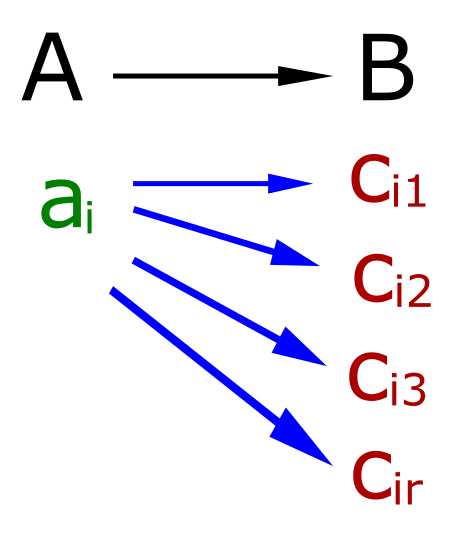
\includegraphics[scale=0.5]{cap02/ImagenNoAplicacion}
	%\includegraphics[width=\textwidth, scale=0.3]{Funcion_hx_002_v4}
	%\includegraphics[width=\textwidth, scale=0.3]{Funcion_hx_001_v4}
	\centering
\end{figure}\\
%\noindent%
%$i \in I=\{ 1, 2, ..., r, ...\}$\\%

En este caso partimos de una simple correspondencia, pues desde que $r\geq 2$ no sería aplicación. Pero tendríamos que $|A| \ngtr |B|$ pues de cada $a_{i}$ sale al menos una flecha, por tanto el número de elementos de $B$ es, al menos, el mismo que el de $A$. Recordemos la regla que obliga a todos los $b_{i}$, a ser todos disjuntos entre sí.



%\newpage%
\section{Interpretación intuitiva}
Un buen ejemplo sería un cine infinito, con sus clientes, o un gallinero infinito con gallinas mutantes que han puesto infinitos huevos.

En el ejemplo del cine con butacas y clientes infinitos, nos daría igual el cardinal de cada conjunto. Simplemente sabiendo, que cada uno, de todos los posibles clientes, tiene tres butacas para su uso absolutamente exclusivo, podríamos afirmar que el cardinal del conjunto de clientes, no es mayor que el cardinal del conjunto de las butacas. Daría igual si fuesen 3, 4, o infinitas butacas de uso exclusivo.

En el caso del gallinero, partimos de un gallinero infinito, con infinitas gallinas mutantes, que la noche anterior pusieron infinitos huevos. Sabemos con absoluta seguridad que todos los huevos tienen dos yemas cada uno. Por lo tanto, podemos afirmar con total tranquilidad, que el cardinal del conjunto de los huevos puestos ese día, no es mayor, que el cardinal de las yemas, de los huevos puestos ese mismo día.

En ninguno de los dos casos, necesitamos preguntarnos que cardinal transfinito tiene cada conjunto.\\\\

$\langle$Comentario Complementario: $\langle\langle$1:Lo que pretendo que se deduzca$\rangle\rangle$

\newpage
\section{Equivalencias con el concepto de inyección}

El Teorema CA, ha acabado siendo una generalización no intencionada de la función inyectiva. Igualmente lo usamos para poder afirmar que el cardinal de un conjunto, no es mayor que el cardinal de otro conjunto. La inyectividad, es un caso particular del teorema.

Pero ahí se acaban las similitudes... Sería un error estar buscando constantemente la alternativa inyectiva de las relaciones que usemos. Lo que buscaremos será abusar y retorcer, las capacidades de las propiedades de los Packs con cardinal transfinito.

Hasta tal punto, que dónde matemáticamente fracasan los conceptos de inyectividad o biyectividad, los Packs transfinitos generarán fenómenos numéricos innegables. Fenómenos que espero generen muchas dudas como mínimo.